\chapter{BACKGROUND}\label{chapter:background}
This chapter describes the context of the thesis from two different perspectives. First, three sections of the chapter concentrate on general testing and tightly related management subjects. Forth section, on the other hand, concentrates on the background of the case at hand.

\section{General concepts in software engineering}
During this section, general concepts related to software testing are laid out. The first subsections holistically describe software quality and testing, while later subsections concentrate on more specific subjects.

\subsection{Quality}
Software quality is hard to define, but its absence is easy to recognise \cite{kitchenham1989software,gillies2011software}. Because of the prior statement, concrete examples can make the essence of the quality easier to understand. For example, a person and her friend are about to buy two public transportation tickets via a new application that the person has just downloaded. In the beginning, the person setups the destination by inputting the address she wants to reach. After inputting the address, she is ready to pay for the tickets.

Unfortunately, while paying for the tickets, the person encounters two problems. The payment button is greyed out, and she does not see an option to buy two tickets. After a while, the person discovers that age and payment options need to be set, which is why she cannot buy a ticket. She cannot find any solution for buying two tickets simultaneously, so she has to buy one ticket at a time. In the end, the first purchase goes through without issues, but the second purchase fails due to an unknown error.

At first, it can be hard to pinpoint precisely, what is wrong, but after some thinking, the problems are apparent. \gls{ui} is hard for a new user to use because the default values of the application are illogical and should be revisited. Wrong default values lead to bad \gls{ux}, finally leading to a lousy quality impression on the user's end. On the other hand, the user would have liked to buy two tickets instead of only one but could not do so quickly. The need for an important feature again reduces the user's quality impression. Finally, the failure of the second ticket is the result of the bad quality.

\begin{minipage}{\textwidth}
	According to \citeauthor{gillies2011software}, the quality can be described via the following five statements \cite{gillies2011software}:
	\begin{enumerate}[noitemsep]
		\item\label{quality1} Quality is not absolute. Considering the above example, some may consider the quality of the software good and instead blame themselves for making mistakes.
		\item\label{quality2} Quality is multidimensional. For example, the above paragraph did have two dimensions, usability of the \gls{ui} and correctness of the functionality.
		\item\label{quality3} Quality is subject to constraints. The application described in the above example may have had a small budget, and it could not be tested sufficiently extensively.
		\item\label{quality4} Quality is about acceptable compromises. Even though there may have been a tight budget with the example application, and the \gls{ux} could have been better, at least the first purchase worked well.
		\item\label{quality5} Quality criteria are not independent. Probably in the above example application, it would have been possible to add an option to buy more than one ticket. However, that would have caused a quality paradox because the application would have become more complex, which was a problem with payment.
	\end{enumerate}
\end{minipage}

Quality also has other definitions. Generally, \gls{iso}9001:2008 states that quality can be determined by comparing intrinsic characteristics with the requirements and that the quality is achieved if the set requirements are achieved \cite{iso9001}. \citeauthor{petrasch1999definition}'s definition of quality is similar to \gls{iso}9001's specification, but has some supplements. In addition to \gls{iso}9001, \citeauthor{petrasch1999definition} states that quality can also be affected by other characteristics not directly related to the requirements \cite{petrasch1999definition}. By this definition, it is inferred that requirements only partially account for all the aspects that may affect the quality. \citeauthor{garvin1988managing} splits quality into five views: transcendental, user, manufacturing, product, and value-based view \cite{garvin1988managing}. These different views emphasise certain aspects of the quality. For example, value-based quality emphasises the monetary value the customer is willing to pay for the product \cite{garvin1988managing}. Overall, quality has plenty of definitions that all hold part of the full definition.

\subsection{Quality assurance}\label{subsection:quality_assurance}
\gls{ieee} defines \gls{qa} as a systematic pattern of actions necessary to provide confidence that an entity conforms to requirements \cite{ieee1990glossary}. \citeauthor{galin2004software} expands \gls{ieee}'s definition by including non-technical development aspects like scheduling and budget \cite{galin2004software}. He also includes quality-related activities during the maintenance of already-released software. On the other hand, software quality also has practical definitions. \citeauthor{tian2005software} defines \gls{qa} as activities that make sure that few or no defects remain in the final software before it is released to the market \cite{tian2005software}.

As a current \gls{qa} professional, I define QA as a set of activities that aim to make software and processes around it as good as possible. In practice, \gls{qa} is carried out by testing the software using various methods, assessing its development and processes professionally, and monitoring test automation results. Targets of the \gls{qa} can vary, but a generally good target for a \gls{qa} professional is to try to assure the quality from the customer's perspective.

The mindset of the \glspl{qa} professionals is different compared to most of the other \gls{pd} staff, like developers. While \glspl{qa} have critical eyes, pay attention to details and concentrate on finding problems, developers, on the other hand, focus on designing and building the software \cite{olsen2018istqbFoundation}. During daily work, the mindset difference is significant. For example, during the security vulnerability research, it was found that security problems were found more effectively if a developer had a more open mindset by nature or if there was a separate team for assessing the security matters \cite{oliveira2018blindspots}. Developers generally trust their code, but due to the developer's confidence, their code may still contain bugs \cite{beck2000extreme}. To avoid some bugs second critical opinion, for example, from the \gls{qa}, is a welcome addition to the development.

\subsection{Software testing}\label{subsection:software_testing}
According to \citeauthor{ammann2016introduction}, software testing is an activity during which it is verified that the software works correctly or according to its specification by running the software and examining the outcomes \cite{ammann2016introduction}. Based on the source, in addition to verification, testing also includes validation activities to ensure that the software specification is appropriate. Based on the \citeauthor{olsen2018istqbFoundation}'s definitions, one of the typical objectives of software testing is to find defects and failures \cite{olsen2018istqbFoundation}. However, the authors also state that the testing cannot prove the absence of defects and is not proof of software correctness. Additionally, \citeauthor{olsen2018istqbFoundation} emphasize that exhaustive testing is impossible. Exhaustive testing is impossible because computer programs are complicated, and testing every scenario would require too many resources.

\subsection{Test automation}
\citeauthor{sharma2014quantitative} states that software testing can be divided into two primary modes: manual testing and automated testing \cite{sharma2014quantitative}. In manual testing, test cases are done manually by the test engineer. In automated testing, test cases are carried out automatically by machines and are built using the help of programming languages according to \citeauthor{sharma2014quantitative}. Because machines cannot currently do abstract reasoning, only verification activities of the software testing can be currently done using automated testing based on the \citeauthor{karhu2009empirical}'s work \cite{karhu2009empirical}. \citeauthor{karhu2009empirical} further lists the advantages and disadvantages of test automation in the paper. The main advantage of automated software testing is increased testing speed due to computers' superior execution speed. At the same time, a significant disadvantage is the increased costs because of the new maintenance, implementation and training requirements.

\subsection{Different levels of testing}\label{subsection:different_levels_of_testing}
According to \citeauthor{black2007pragmatic}, V-model seen in the \autoref{fig:v-model} is an upward bend testing-focused version of the commonly known waterfall software model \cite{black2007pragmatic}. The model emphasises that more straightforward tests, like unit tests, focus on lower-level details while higher test levels concentrate on more complex topics based on the paper. From another point of view, the V-model can also be seen as a relation between requirements and testing \cite{dick2017Requirements}. Even though in the \autoref{fig:v-model}, requirements are only tied to the user acceptance level testing, requirements can also be considered to be directly tied to other testing levels. For example, subsystem requirements can be directly related to the integration testing \cite{dick2017Requirements}. More information about testing levels is available in the \autoref{section:technical_background}.
\begin{figure}
	\includegraphics{V-model}
	\caption{V-model \cite{macario2013test}}
	\label{fig:v-model}
\end{figure}

\section{Management background}
The background of the \gls{ta} management-related matters will be described in this section. The section includes multiple sub-sections describing the test automation management background from different perspectives. The first two subsections are related to the introduction of test automation. The third subsection tells about test automation-related education aspects, and the last two subsections describe daily activities of the test automation development.

\subsection{Introduction of the test automation}
Before test automation can be deployed properly, there must be a plan for how the test automation will be taken into use appropriately. Generally, there are four steps during the introduction process. The steps are 1) team assembly, 2) publicity, 3) test automation pilot and 4) phased implementation of the test automation \cite{fewster1999software}. There is also a more fine-grained 10-part introduction process, which includes phases for test strategy, test tool compatibility and training requirements \cite{dustin1999automated}. This process fits the previously defined introduction process framework reasonably well but is considerably more detailed. An alternative, more practical definition of the introduction process is 5 step \gls{ast} process. The process steps are 1) requirements gathering, 2) case design and development, 3) automation framework development, 4) test execution and reporting and 5) program review and assessment \cite{dustin2009implementing}.

In addition to the introduction processes, introduction roles should be acknowledged before beginning the test automation preparations. According to one definition, these roles could be: \gls{ta} tool selection champion, organisation change agent, management sponsor, \gls{ta} tool customiser and implementation team members \cite{fewster1999software}. These roles, especially organisation change agent and management sponsor, would activate the company's management into what is necessary for the project's success of the project \cite{fewster1999software,graham2012experiences}.

\subsection{Prioritisation of the test automation}\label{subsection:prioritization_of_the_test_automation}
When the new test automation system is used, it is crucial to understand which parts of the system on which testing level should be automated first so that the test automation system advantages can be maximised from the start. As a starting point, it has been recommended that the test cases that are boring to perform and repetitious or very complex to execute manually should be automated first \cite{graham2012experiences}. Test cases that are executed often and require large amounts of data should also be among the first to be automated \cite{gaur2012automated}. From the financial perspective, test cases with the highest \gls{roi} should be automated first \cite{graham2012experiences}.

While considering the test automation prioritisation, it is good to consider the required automation test case efforts. Test cases with low effort and high value should have top priority when automating the test cases \cite{gunasekaran2015survey, fewster1999software}. However, this balance may be hard to achieve because, for example, unit tests are easy to create, but they cover only a tiny part of the application. On the other hand, integration and system tests cover a more significant part of the application, but they are harder to construct. In practice, more complex smoke and integration tests have been observed to offer better \gls{roi} \cite{berner2005observations}.

\subsection{Test automation education}
Before the test automation system can be taken into use, developers must be aware of the test automation development and the best practices. It has been stated that automation education is often the key to successful automation because people often need help understanding what is realistic with the automation and what is not \cite{graham2012experiences}. However, during a survey, it was discovered that only 38\% of the respondents felt that sufficient test automation education had been provided to them \cite{sundaralingam2021analysis}.

According to \citeauthor{timoney2008experiences}, test automation has been seen as a tricky subject to educate in universities because test automation requires a significant amount of prior knowledge, for example, from fundamental software testing and software modelling \cite{timoney2008experiences}. In addition, it has been stated in the paper that recommended test automation tools have constantly been fluctuating, making it hard to find a good test automation tool suitable for education. So, education about the test automation tool is crucial, but general knowledge about the testing should be appropriate. Based on the context of this thesis and based on the following three books \cite{ammann2016introduction, everett2007software, singh2012software} \glspl{toc} for example, the following topics could be covered during the test automation education sessions:
\begin{itemize}[noitemsep]
	\item What is software testing?
	\begin{itemize}[noitemsep]
		\item Why do we test software?
		\item Objectives and limitations of Testing
		\item The value versus the cost of testing
	\end{itemize}
	\item Testing types
	\item Psychology of testing
	\item Software test automation
\end{itemize}

\subsection{Test automation daily development activities}\label{subsection:test_automation_daily_activities}
In the \citeauthor{royce1987managing}'s paper classical "waterfall model" is introduced, which is a linear process model for software development \cite{royce1987managing}. The model has roughly the following phases: 1) requirements, 2) preliminary design, 3) analysis, 4) program design, 5) coding, 6) testing and 7) operations. Notably, in the model, software testing has been placed as a second last step right before the step during which software is taken into daily use. However, even in the original \citeauthor{royce1987managing}'s paper defining the "waterfall" process, it was noted that placing the testing as one of the final steps of the process is risky. According to \citeauthor{royce1987managing}, situating testing among the last steps is risky because all the possible design issues that may cause significant redesign would be detected late. Due to the waterfall process's inherent problems, nowadays, agile processes are used more commonly instead. The agile process has many principles, but one of the main principles is "Responding to change over following the plan" \cite{beck2001agile}. The agile process premise differs significantly from the waterfall process' premise.

Currently, the most popular agile process is the Scrum process, used even by 94\% of the teams using Agile processes \cite{rubin2012essential, scrum2018state}. \citeauthor{rising2000scrum} describes Scrum as an incremental process for building software in complex environments while staying at the edge of the developing organization's tolerances \cite{rising2000scrum}. \citeauthor{rubin2012essential} defines the Scrum process as follows \cite{rubin2012essential}. In the Scrum process, the software is developed in small iterations called sprints instead of one monolithic development pipeline. During the iteration, new features and bug fixes are made to the software, and those improvements are tested. Finally, at the end of the sprint, during a sprint review, it is verified using \gls{dod} that the new improvements have been made appropriately and development included proper testing of the improvements.

One alternative agile approach to Scrum process is \gls{xp}. In \gls{xp} process, testing is defined to be isolated and automated. Test cases are written by programmers and customers \cite{beck2000extreme}. Compared to the Scrum process, the \gls{xp} process explicitly defines how testing practices work. However, both processes agree that test automation should be an integral part of the development activities.

In addition to overall development process frameworks, a process for writing the test cases is also important. Traditionally the automation test cases have been written after the code has been constructed in a waterfall-like fashion. Nowadays, it is popular to use \gls{tdd} instead \cite{jorgensen2013software}. In \gls{tdd}, test cases are written before the code \cite{beck2003test}. It has been stated that when using \gls{tdd}, the program is always working, but possibly in an incomplete state \cite{jorgensen2013software}. \gls{tdd} follows the following three-step process, red: write a test that does not work, green: make the test work by any means necessary, refactor: improve the code by removing dirty solutions done during the previous step \cite{beck2003test}. \gls{xp} uses \gls{tdd} explicitly \cite{beck2000extreme}.

\subsection{Test automation roles}\label{subsection:test_automation_roles}
Based on the mentioned agile processes, it can be stated that the developers should write test automation cases and, in some cases, possibly even the customers \cite{rubin2012essential, beck2000extreme}. Additionally, domain experts can help with the writing of the test cases \cite{winkler2018towards}. However, according to \citeauthor{ieshin2009test}, it is not recommended that the whole test automation stack is developed by the same team that develops the test cases \cite{ieshin2009test}. Instead, in the \citeauthor{ieshin2009test}'s paper, it is recommended that companies should have a centralised \gls{taf} team to avoid problems like fragmentation of knowledge, redundant work and too small resources for \gls{ta}. \citeauthor{graham2012experiences} state that from the management point of view most important responsibility is to provide sufficient support and resources for the test automation efforts \cite{graham2012experiences}. They further emphasise that sufficient management efforts are vital for test automation's success.

Additionally, as part of the test automation process, there can be a test manager who manages the big picture of the test case creation and supervises the test reports produced by the test automation \cite{winkler2018towards}. The team leaders lead practical work of the test automation \cite{pol2002software}. Team leaders have different names and slightly different responsibilities based on the selected, overall development process model. For example, in Scrum, Scrum master could be classified as a team leader who oversees the current development activities, including testing \cite{rubin2012essential}. Test automation engineer can also be considered as a separate role \cite{pol2002software}. Test automation engineers are vital for the \gls{taf}, which requires an excellent knowledge of test automation.

\section{Technical background}\label{section:technical_background}
This section introduces different test levels and technologies from the test automation point of view. The first five subsections describe testing levels introduced in the \autoref{subsection:different_levels_of_testing}, while the last section describes the basics of the \gls{ci}.

\subsection{Unit testing}\label{subsection:unit_testing}
Unit tests are simple sanity checks for the code, and they are used to evaluate if the results of the computations are correct swiftly \cite{acharya2014mastering}. The purpose of the unit tests is to check that code being written during feature development is correct \cite{simon2014mastering}. From the architectural standpoint, unit tests help ensure that developed code is appropriately decoupled according to \citeauthor{khorikov2020unit}'s paper \cite{khorikov2020unit}. The paper further states that unit tests are crucial for the software project because they enable sustainable project growth via positive architectural improvements.

The scope of the unit test is the tiniest functional point, which is often a single class \cite{huizinga2007automated}. The alternative \citeauthor{osherove2013art}'s scope definition describes that the unit tests are used for testing the units of work \cite{osherove2013art}. Units of work are behaviours that can be initiated via public \glspl{api}, and the effect of the initiation can be observed via some externally visible result like a return value based on the work. While the first definition implicitly restricts a single unit test to an instance of the class, the alternative definition explicitly allows unit tests to span multiple classes if it is deemed necessary for the one unit of work \cite{huizinga2007automated, osherove2013art}.

One great approach for unit testing is \gls{aaa} pattern invented by \citeauthor{wake2011aaa} \cite{wake2011aaa}. In the \citeauthor{simon2014mastering}'s book, \gls{aaa} pattern is described as follows. During the arrange phase, the test scenario is set up, fake objects are prepared, and an instance of the class under testing is created. In the act phase method under testing is executed. Finally, in the assert phase, it is made sure that the program's state is as expected. In the simplest case, an assertion can consist of checking the function's return value as hinted in the unit of work \cite{osherove2013art} definition.

Act and assert phases are often relatively straightforward in the \gls{aaa} pattern, but surprisingly, the arrange phase can be pretty complex in unit testing due to the need for fakes. Fakes are objects with limited functionality and are used in testing in place of the actual objects to limit a unit test to only a particular part of the program \cite{simon2014mastering}. Fakes can be classified into subcategories, such as stubs and mocks \cite{simon2014mastering}. Stubs replace the functionality of the original method with something more suitable for testing, while mocks additionally verify already during runtime that the replaced method is called with the correct arguments \cite{ammann2016introduction}. So basically, mocks are stubs but with built-in assertions.

While unit testing is a helpful tool, it has its challenges. According to \citeauthor{runeson2006survey}, it can be hard to decouple different units, and unit tests may, in the end, test too much \cite{runeson2006survey}. Additionally, as a related problem, units with large data structures are hard to unit test. \citeauthor{hunt2003pragmatic} states in their book that many tests can break, because of the modifications to the functionality, if the code under testing is highly coupled \cite{hunt2003pragmatic}. They also state that tests may fail on some machines if the test code contains any timing problems. In addition, generally \gls{ui} related unit testing is seen hard \cite{runeson2006survey}.

\subsection{Integration testing}\label{subsection:integration_testing}
According to \citeauthor{brar2015international}'s paper, integration testing verifies that the units tested during the unit testing work also correctly with each other in addition to working alone \cite{brar2015international}. The paper also describes the advantages and disadvantages of integration testing. Integration testing's advantage compared to unit testing is that it is more capable of discovering problems. However, a downside of this is that it is more challenging to find the root cause of the problem based on the integration testing results. In addition, integration tests are generally slower to run than unit tests \cite{simon2014mastering}.

Based on the \citeauthor{olsen2018istqbFoundation}'s syllabus, integration testing is divided into component and system integration testing \cite{olsen2018istqbFoundation}. The syllabus further defines that in component integration testing, it is verified that integrations between internal software components work correctly. On the other hand, system integration testing concentrates on testing interfaces between different systems. One of the most common challenges in component integration testing is that \gls{cots} components are hard to test with due to lack of source code visibility \cite{rehman2006software}. Similar problems may also arise with the system-level integration testing if the commercial software systems' documentation only includes some essential details.

Integration testing can be done using one of the four approaches: 1) top-down, 2) bottom-up, 3) threaded integration/sandwich and 4) big bang. The difference between the methods is the order of integration. In the top-down higher-level components are tested first together before lower-level components, while in the bottom-up approach, it is another way around. Threaded integration, on the other hand, is a combination of the previous two. In the big bang method, all the units are integrated at once. \cite{brar2015international, uma2013software, singh2012approach}

One form of integration testing is \gls{api} testing \cite{vu2018automation}. According to \citeauthor{isha2018automated}'s paper, in \gls{api} testing, an application's often \gls{rest} based \glspl{api} functionality is tested \cite{isha2018automated}. Additionally, it is stated in the paper that \gls{api} testing is often done automatically because manual \gls{api} testing is time-consuming, error-prone and impossible for the \gls{api} endpoints with more extensive data flows. As stated by \citeauthor{bangare2012automated}, in \gls{api} testing \glspl{api} can be treated as black boxes \cite{bangare2012automated}. However, the article also mentions that this approach may leave some code paths inside the application untested. Due to this, unit tests that are closer to the source code are still useful.

Because integration tests are testing larger bodies of applications, integration tests may require more complex preliminary preparations. For example, a test database that can be restored to a known state is often needed in integration testing \cite{bangare2012automated}. Integration testing also has other challenges. One of the most prominent problems of integration testing is test flakiness, which reduces developers' trust in automation testing and causes significant computing overhead \cite{micco2017state}. Flaky tests are non-deterministic test cases that sometimes fail by themselves \cite{bell2018deflaker}. Additionally, software component heterogeneity, constantly fluctuating code base and lack of information caused by the lack of access to source code for the commercially available components are seen as impediments to the integration testing \cite{rehman2006software}.

\subsection{System testing}\label{subsection:system_testing}
System testing is a testing level that focuses on a system as a whole and aims to verify that specified requirements are met \cite{istqb2018system}. Unlike integration testing, system testing does not require knowledge about the application's inner workings \cite{bangare2012automated}. Because of this, manual testing is often done on the system testing level by the \gls{qa} engineers. In addition to functional testing, system testing also includes qualitative testing activities, like, for example, performance testing \cite{binder2000testing}.

One form of system testing is \gls{gui} testing \cite{borjesson2012automated}. In \gls{gui} testing, sequences of user input events are executed against a \gls{gui} \cite{banerjee2013graphical}. \gls{gui} testing is probably the most common type of system testing because most new applications contain some forms of \glspl{gui}. The existence of \gls{gui} is problematic for the applications' creators because \glspl{gui} are complex and expensive to test \cite{miller2001acceptance}.

One technique for \gls{gui} testing is \gls{vgt} \cite{borjesson2012automated}. \gls{vgt} based techniques speed up error-prone manual testing activities. However, \gls{vgt} has challenges like lack of empirically-based knowledge and associated costs \cite{alegroth2015visual}.

As with other testing levels, system testing has its challenges. For example, regarding \gls{gui}, testing synchronisation of the user actions and recognition of the \gls{ui} objects can be challenging according to \citeauthor{graham2012experiences}'s book \cite{graham2012experiences}. Furthermore, it is stated in the book that automation test tools do testing differently compared to humans, which causes unexpected behaviours in the application. Probably partly due to these problems, the usability of the test tools has been seen as the most crucial criterion during tool selection \cite{paivi2017choosing}.

\subsection{User acceptance testing}
During \gls{uat} user checks produced software to accept it \cite{pandit2015agileuat}. Unlike during system testing, \gls{uat} is tested in a production-like environment \cite{otaduy2017user}. The end goal of the \gls{uat} is to establish confidence in the user that the produced software is fit for the purpose \cite{pandit2015agileuat}. \gls{uat} will not be addressed further in this thesis because it is out of scope.

\subsection{Continuous integration}
\glsfirst{ci} is a development practice in which application developers integrate their development work often \cite{fowler2006continuous}. Originally \gls{ci} was invented as a part of the \gls{xp} software process framework, but later it has also been used outside of it \cite{meyer2014continuous}. \gls{ci} is often exercised with the help of automation, which verifies that the software can still be successfully built and that the automated test cases do pass \cite{fowler2006continuous}. The advantage of \gls{ci} practices is that they do effectively prevent: "it works on my machine" syndrome, and that way reduces the risk of taking code into production \cite{meyer2014continuous}.

\section{Context of the project}\label{section:context_of_the_project}
This section describes the context of this project by describing companies and products around it. The first section introduces the parent company M-Files. After the introduction of the M-Files, the Hubshare division is introduced. Finally, Hubshare as a product is presented.

\subsection{M-Files Oy}
M-Files Oy is a Finnish software company that has over 500 employees around the world. M-Files' headquarters is located in Tampere, Hervanta, Finland, but M-Files also has offices in the United States, Great Britain and France. The company currently has over 5 000 customers in over 100 countries worldwide. \cite{mfiles2022tutustu}

Nowadays, M-Files' mission is to boost companies' business activities in the current location-independent world. The company has a core product, which is also called M-Files. M-Files is a smart information management platform which helps companies manage information more efficiently and automate business processes. M-Files product \gls{ui} can be seen in the \autoref{fig:m-files_interface}. \cite{mfiles2022tutustu}
\begin{figure}
	\centering
	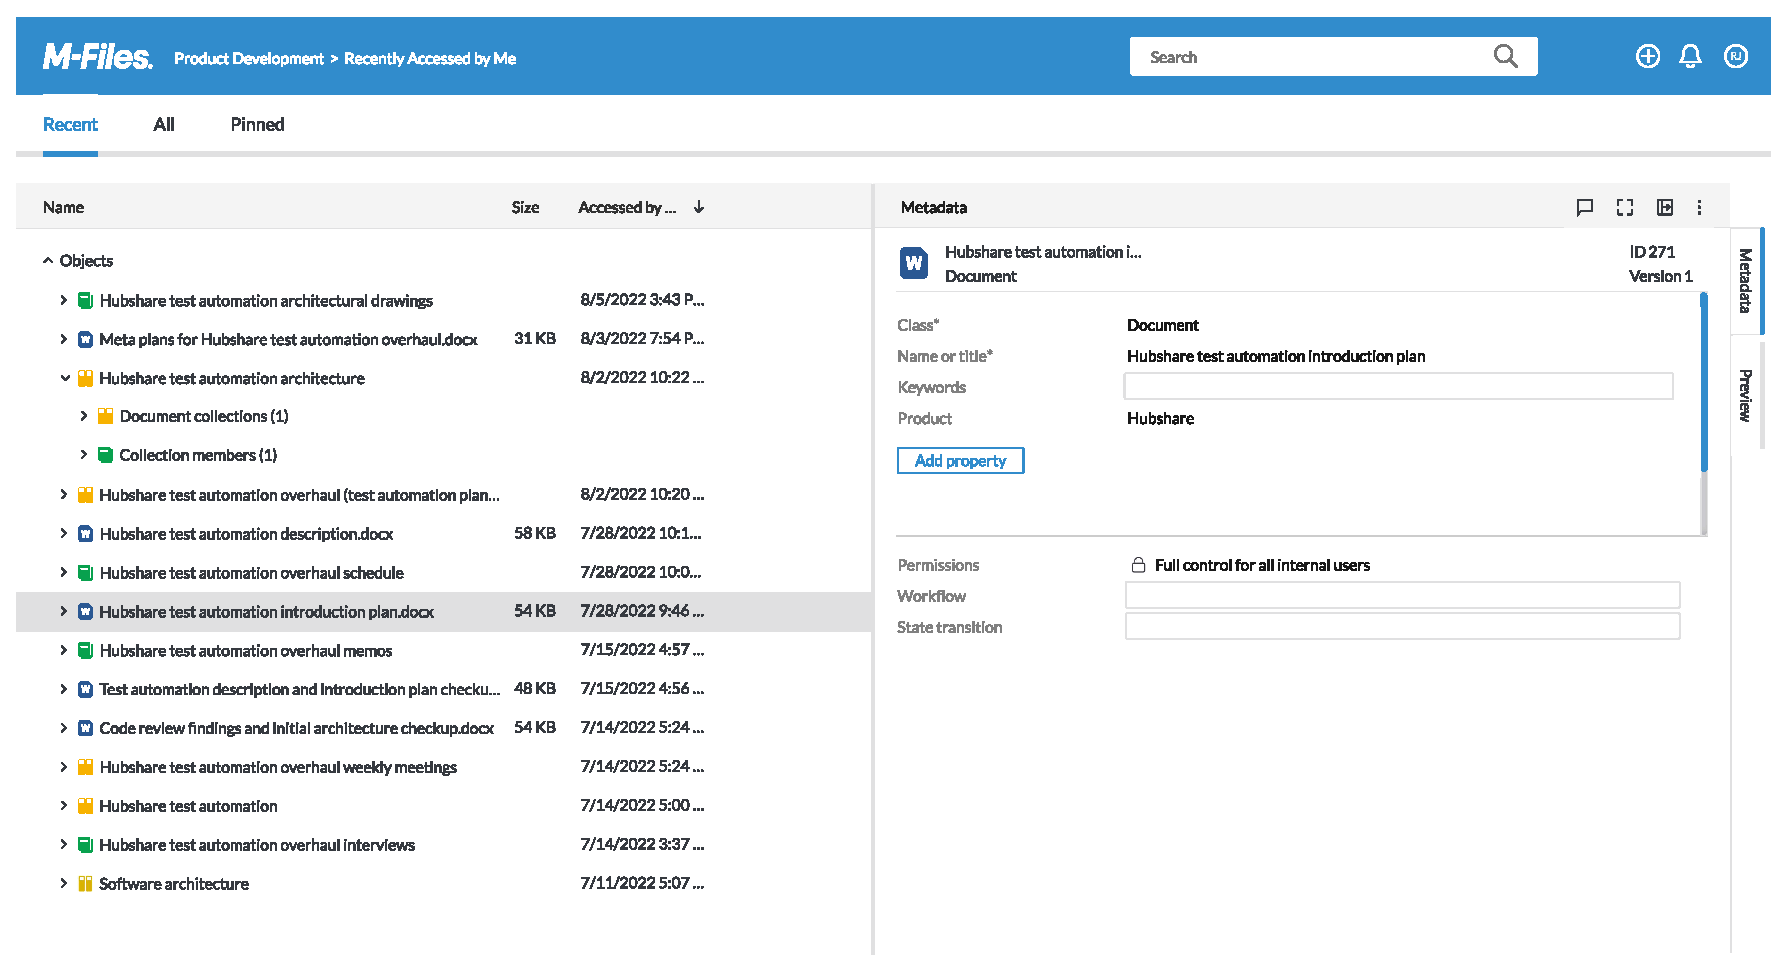
\includegraphics[width=0.7\textwidth]{M-Files_interface}
	\caption{M-Files Web \gls{ui}}
	\label{fig:m-files_interface}
\end{figure}

M-Files started as Motiivi Oy in 1987, later known as Motive Systems and M-Files. Business related to the M-Files product started in 2002. The First version of the M-Files was released in 2005. After that, M-Files has grown fast, even 40-50\% per year. \cite{mansikkamäki2017tamperelainen, pääomasijoittajat2022mfiles}
\FloatBarrier

\subsection{Hubshare division}\label{section:hubshare_division}
Hubshare started as an independent software company in 1997 but was later acquired by M-Files in 2021 \cite{hubshare2020, dekelbaum2021mfiles}. Before its acquisition, Hubshare specialised as a reseller of software solutions for legal companies and professionals. In 2013 they started creating their main product Hubshare \cite{hubshare2020}. Nowadays, Hubshare is part of the M-Files company and develops and provides its main product, Hubshare, alongside the M-Files platform portfolio \cite{dekelbaum2021mfiles}.

\subsection{Hubshare as a product}\label{section:hubshare_as_a_product}
Similarly to M-Files, Hubshare's main product shares the name with the company and is called Hubshare. According to Hubshare's technical manager, Hubshare is a SaaS web platform that allows users to collaborate with internal and external stakeholders around documents, projects, events and all other information beneficial for their business. In practice, Hubshare is used for creating customisable intranets, and extranets for companies \cite{mfiles2022Hubshare}. Hubshare \gls{ui} can be seen in the \autoref{fig:hubshare_interface}.
\begin{figure}
	\centering
	\includegraphics[width=0.7\textwidth]{Hubshare_interface}
	\caption{Hubshare's dashboard interface}
	\label{fig:hubshare_interface}
\end{figure}